\documentclass[10pt,a4paper]{article}

\usepackage[utf8]{inputenc}
\usepackage[spanish]{babel}
\usepackage{amsmath}
\usepackage{amsfonts}
\usepackage{amssymb}

\usepackage{color} %Use custom colors and give color to text
\usepackage{graphicx} %Include images
\usepackage{float}
\usepackage{subfig}
\usepackage{enumerate}

\usepackage{multirow}
\usepackage[table,xcdraw]{xcolor}

\usepackage{hyperref} %referencia

\author{\textbf{Gustavo Rivas Gervilla}}
\title{\textcolor{deepblue}{\textbf{Lógica difusa para la descripción de datos}}}
\date{}

%Custom colors
\definecolor{deepblue}{rgb}{0,0,0.5}

%Custom itemize bullet
\def\labelitemi{$\blacktriangleright$}

\newtheorem{definicion}{Definición}
\newtheorem{proposicion}{Proposición}

\begin{document}
\pagenumbering{gobble} %turn off page enumeration
\maketitle
\begin{center}

\includegraphics[scale=0.5]{img/decsai}
\end{center}

\newpage

\tableofcontents

\newpage
\pagenumbering{arabic} %turn on page enumeration
\section{Introducción}

Actualmente existe una gran cantidad de información que nos llega en distintos formatos. Por ejemplo nos pueden llegar en forma de tabla o forma de serie temporal. En caso de ser usuarios expertos podremos trabajar con estos datos y obtener las conclusiones que necesitemos para completar la tarea que estemos abordando, por ejemplo aplicando técnicas de minería de datos en caso de que poseyamos el conocimiento necesario para ello.\\

Pero la información no siempre va destinada a usuarios expertos con lo realizar una análisis de los datos en bruto para obtener una información que les sea de utilidad puede resultar muy complejo o imposible para ellos. Así que elebarorar una descripción linguística en forma de texto compresible por el usuario de los datos se ha convertido en los últimos tiempos en algo fundamental.\\

Hoy en día, la tarea de generar información intendible por los usuarios usando lenguaje natural (que es al fin y al cabo el que maneja el usuario en su día a día) ha sido abordada desde dos campos: el de la generación de languaje natural (\textbf{NLG}, por sus siglas en inglés) y el de la descripción lingüística de datos (\textbf{LDD}, por sus siglas en inglés). Pese a que estos dos campos son en inicio independiente la tendencia que están siguiendo el avance en ambos los llevará finalmente a converger.\\

El campo de la NLG se centra en la creación de textos que proporcionan información contenida en diversos formatos con el propósito de que esos textos sean indistinguibles, tanto como sea posible, de uno creado por humanos. Por el otro lado, el campo de la LDD, que aparece como un a de las principales aplicaciones de la \textbf{teoría de conjuntos difusos}, proporciona resúmenes o descripciones de conjuntos de datos empleando conceptos lingüísticos definidos en forma de conjuntos difusos y particiones difusas, lo que le permite tratar con la imprecisión inherente al lenguaje natural. Aquí se remarca una capacidad muy importante de los conjuntos difusos y es que nos permiten representar conceptos que no tienen una definición precisa y que están sujetos a la subjetividad de cada persona.\\

El campo de la NLG es más antiguo que el de la LDD, este campo comenzó a desarrollarse en los 80, y pese a tener ya un tiempo de desarrollo continúa siendo un campo de investigación abierto en muchos aspectos y no hay una técnica única para abordar los problemas de generación de lenguaje natural.\\

Por otro lado la descripción lingüística de datos trata de obtener descripciones concisas e informativas de \textit{datasets} numéricos y cubre un grupo de técnicas basadas en soft computing, como las variables lingüísticas o los cuantificadores y operadores difusos. Este campo comenzó a desarrollarse con fuerza a mediados de los 90 con el avance en el campo de los conjuntos difusos, dando lugar a nuevas aplicaciones en el enfoque descriptivo del \textit{data mining}.\\

\subsection{NLG}

John Bateman describió la generación de lenguaje natural como la rama del procesamiento de lenguaje natural que trata el problema crear automáticamente con una máquina textos en lenguaje natural.\\

La demanda de textos en lenguaje natural que proporcionen todo tipo de información está aumentando actualmente. Algunos ejemplos que podemos destacar de la NLG son \textbf{genración de partes meteorológicos en diversos idiomas a partir de datos meteorológicos}, \textbf{generación de cartas de respuesta a clientes}, \textbf{generación de informes sobre el estado de recien nacidos}. Pese a que nosotros queremos hablar sobre aplicaciones de la lógica difusa en descripción lingüística de datos, comentamos estas aplicaciones ya que como te comentó anteriormente y teniendo en cuenta que en este tipo de aplicaciones se trabaja con conceptos procedentes del lenguaje natural; más tarde o más temprano la lógica difusa enriquecerá y potenciará todas las aplicaciones que hemos enumerado.\\

A continuación vamos a dar una pequeña descripción de cómo se diseña un sistema de NLG, ya que algunas de las fases que vamos a enumerar tendrán su correspondencia con el diseño de la aplicación final que vamos a comentar.

\subsubsection{Diseño de un sistema de NLG}

El diseño de un sistema de generación de lenguaje natural es algo abierto en la que no hay una guía concreta que seguir. Dependerá del propio diseñador y del problema a resolver. No obstante podemos desglosar la tarea principal que afrontará cualquiera de estos sistemas (convertir unos datos de entrada en un texto) en una serie de tareas que podríamos considerar, en mayor o menor medida, como comunes a todos los sitemas de NLG:

\begin{itemize}
\item \textbf{Determinación del contenido:} decicir qué información se ha de comunicar por medio del texto a crear.
\item \textbf{Planificación del discurso:} dar un orden y una estructura al conjunto de mensajes a verbalizar.
\item \textbf{Agrupación de oraciones:} agrupar varios mensajes en una sola oración. Esta tarea no es siempre necesaria, en tanto en cuanto cada mensaje puede ser expresado por medio de una oración de forma individual.
\item \textbf{Lexicalización:} decidir que palabras y expresiones han de usarse para expresar los conceptos y relaciones del dominio que aparecen en los mensajes.
\item \textbf{Geración de las expresiones de referencia (referring expression):} seleccionar las palabras o expresiones que identifican las entidades del dominio. Aunque puede parecer una tarea similar a la anterior, en este caso buscamos discriminar cada entidad del dominio del resto; empleando para ello tanta información como sea necesaria (siempre que se disponga de ella claro).
\item \textbf{Realización lingúística:} aplicar reglas gramaticales para producir un texto que sea sintácticamente, morfológicamente y ortográficamente correcto a partir de los elementos anteriormente generados.
\end{itemize}

\section{LDD}

Este campo, que trata de construir descripciones de datasets empleando términos lingüísticos, surge con las ideas de \textbf{Lofti A. Zadeh} y \textbf{Ronald Yager}, lo cuáles presentaron la lógica difusa como una herramienta para realizar computación desde un punto de vista lingüístico. De estas ideas proviene el paradigma de la computación con palabras (CW, por sus siglas en inglés) y su evolución más moderna, la teoría computacional de conceptos (CTP, por sus siglas en inglés) que, según el propio Zadeh, \textit{añade a los sistemas de computación tradicionales dos importantes capacidades: (a) la capacidad de precisar el significado de las palabras y las proposiciones extraídas del lenguaje natural; y (b) la capacidad de razonar y computar con palabras y proposiciones precisadas}. Aunque han surgido muchas aproximaciones basadas en CW, la más prometedora es el resumen lingúístico de datos, el cual emplean sentencias cuantificadas de forma difusa para obtener resúmenes lingüísticos.\\

Algunos dominios de aplicación en los que se ha aplicado este paradigma es el flujo de entrada de pacientes a un centro de salud, consumo doméstico de electricidad, medición de la calidad de los andares de un individuo, actividad humana basada en acelerómetros del dispositivo móvil o en el terreno de la meteorología.\\

Este es un campo de reciente aparición con lo que encontrar una técnica general capaz de generar distintos tipos de descripciones lingüísticas para cualquier tiene de dominio de aplicación es una tarea aún por completar, aunque ya se han dado algunos pasos en esta dirección. Además también es importante la creación de criterios generales sobre cómo estructuras sentencias cuantificadas para obtener descripciones más complejas o cómo construir y evaluar descripciones lingüísticas. Con lo cual, al igual que sucede en el campo de la NLG, no hay un consenso sobre cómo ha de implementarse un sistema de LDD.

\subsection{Elementos en un enfoque de descripción lingüística de datos}

El proceso de creación de una descripción lingüística puede definirse como la tarea de extraer la información más importante de unos datos de entrada produciendo una abstracción formada por términos lingüísticos. Esto es similar a la fase de determinación del contenido de los sitemas de NLG y constituye el nexo principal entre ambos campos.\\

Pues bien los elementos principales para crear una descripción lingüística son:

\begin{itemize}
\item Los \textbf{datos de entrada}.
\item \textbf{Variables lingüísticas} que se definen en el dominio de la variable de entrada como conjuntos difusos que etiquetan o categorizan ese dominio. Por ejemplo para la variable de entrada \textit{velocidad de conducción} podemos tener las etiquetas lingüísticas: \textit{adecuada, mala o ideal}.
\item \textbf{Cuantificadores difusos}.
\item \textbf{Criterio de evaluación}. El uso de variables lingüísticas y cuantificadores nos posibilitan crear una gran multitud de descripciones diferentes. Por lo tanto se hace patente la necesidad de tener un criterio para elegir la más adecuada entre ellas. Ya veremos más adelante el criterio que se empleó en la aplicación objetivo de mi TFG.
\end{itemize}

Este conjunto de elementos nos sirve para crear las descripciones lingüísticas más simples, las oraciones cuantificadas de tipo I como ``unos poco perros son marrones'' que pueden ser computadas usando un modelo de cuantificación difusa.\\

La construcción de oraciones cuantificadas y, en general, de descripciones lingüísticas, es un proceso que está muy influenciado por las técnicas difusas en las que se basa. Por lo tanto, para manejar la impreción implícita en las variables lingüísticas y las particiones de cuantificación, los algoritmos usados en el campo de LDD generan todas las posibles combinaciones de oraciones para dar lugar a todas las descripciones posibles. Entonces con el criterio de selección comentado anteriormente, todas las descripciones se ordenan y se elige la mejor de ellas, por tanto este proceso podría verse como una búsqueda guiada por la meta, como un algoritmo greedy. Por tanto tantos los algoritmos heurísticos como aquellos que hacen uso de meta-heurísticas se emplean para dirigir el proceso de búsqueda, para no optar por una búsqueda por fuerza bruta; que sería muy ineficiente.\\

\subsection{Técnicas y casos de uso}

Lo que ocurre en el campo de la LDD es que la componente teórica es mucho más fuerte que la práctica, e incluso cuando se presenta una nueva aplicación práctica se emplea mucho lenguaje matemático para formalizar la tarea de la generación de las descripciones lingüísticas.

\subsubsection{Trabajo teórico}

Uno de los principales objetivos que se abordan en este campo es el de diseñar un \textit{framework} que sea aplicable para cualquier tipo de problema de descripción en cualquier dominio, pero aún no se ha logrado alcanzar esta meta. En esta dirección tendríamos el modelo lingüístico granular de un fenómeno (GLMP por sus siglas en inglés), propuesto por Trivino y Sugeno, es una de las aproximaciones más prometedoras en este sentido. Está basado en una jerarquía de nodos interconectados llamados mapeos de percepción (PM por sus siglas en inglés), que reciben un conjunto de percepciones computacionales (CP) como entrada. Cada PM le aplica una función a las CP (por ejemplo el mínimo, el máximo, la media o alguna regla difusa) y genera nuevas CP que pasan como entrada al siguiente nivel de PM. En esta red cada CP cubre ciertos aspectos del fenómeno con un cierto grado de granularidad.\\

Otra nueva contribuciones plantean el uso de nuevos cuantificadores y nuevos métodos de evaluación para sentencias cuantificadas. Por ejemplo Díaz-Hermida explora varios aspectos teóricos como el uso de cuantificadores semi-difusos para modelar sentencias cuantificadas y describe algunos métodos genéricos para la detección de patrones.

\section{Descripción lingüística de series temporales}

En esta sección vamos a ver en algo de más profundidad una de las aplicaciones principales en el campo de la LDD, donde los conjuntos y sistemas difusos hacen aportaciones muy importantes, que la descripción lingüística de series de temporales.\\

Este enfoque se descompone en dos tareas principales, la extracción de conocimiento y un proceso de expresiones lingüísticas. El enfoque que vamos a ver incorpora como un elementos principal un modelo descriptivo el cual tiene tres piezas fundamentales: un mecanismo de formalización del conocimiento, un lenguaje de expresión y un marco de calidad.\\

Muchos profesionales en el área de las TIC tienen la tarea de dar sus usuarios conocimiento útil extraído a partir de un flujo de datos que están en constante crecimiento, en la mayoría de los casos para ayudar en problemas de decisión. En muchas ocasiones estos datos vienen en forma de series temporales, es decir, secuencias de datos procedentes de la observación de un fenómeno que están ordenados en el tiempo. Hay una gran cantidad de aplicaciones de economía, salud cardíaca y bienestar social, entre otros campos, que están relacionadas con la descripción lingüística de series temporales.\\

En muchas aplicaciones o tareas el usuario recibe una gran cantidad de información que se ven a obligados a intentar interpretar, lo cual puede ser un proceso complejo sobre todo para usuarios no expertos. Por otro lado, la interacción persona-ordenador basada en lenguaje natural es un campo que está creciendo en popularidad e importancia en las últimas décadas. Por lo tanto la descripción lingüística de datos es un campo de gran utilidad en la actualidad.\\

Como ya hemos comentado una descripción lingüística de datos expresa conocimiento extraído de datos usando lenguaje natural. La generación lingüística de datos consiste en dos tareas principales: un proceso de extracción de conocimiento que puede ser considera como un proceso de extracción de conocimientos en una base de datos, definido como un adquisición de conocimiento novedoso, útil y fácilmentente entendible a partir de los datos, y por otro lado un proceso de expresión lingüística que intenta mejorar la utilidad del conocimiento extraído y hacerlo más entendible usando lenguaje natural.\\
 
Un sistema de descripción lingüística de series temporales (GLiDTS por sus siglas en inglés) son sistemas computacionales que simulan la respuesta que daría un experto a la pregunta de qué ve o destaca en una serie temporal. Tanto el tipo de descripción lingüística obtenida como las técnicas empleadas para su obtención son muy variadas, incluso dentro del mismo dominio. Por ejemplo, una respuesta distinta se espera para la solicitud \textit{Habláme sobre cómo pasó el paciente la noche pasada}, donde se espera una descripción completa de varias series de datos de monitorización, y \textit{Háblame sobre cambios significativos en el ritmo cardíaco del paciente}, donde el objetivo es localizar segmentos de las series temporales que concuerden con patrones lingüísticos definidos como \textit{aumentando} o \textit{decreciendo rápidamente}.\\

En KDD y Aprendizaje Automático, la teoría de conjuntos difusos tiene el potencial de producir modelos que sean más comprensibles, menos complejos y más robustos, siendo especialmente útiles para representar patrones imprecisos y modelar y procesar varios tipos de imprecisión e información incompleta. En NLG, la teoría de conjuntos difusos tienen una un papel muy importante en dotar de semántica a los datos recibidos como entrada, y tratar con distintos tipos de imprecisión inherente en el lenguaje natural.

\subsection{Generación de descripciones lingüísticas de series temporales}

Ya hemos dicho que el objetivos de los sistemas de GLiDTS es simular la respuesta de un experto. Ahora bien, hay otros dos agentes que son importantes para estos sistemas: el destinatario de la información y el diseñador del sistema. Por lo tanto el proceso de generación de las expresiones lingüísticas para describir la información extraída está influenciada por las características del destinatario.\\

Así los datos recibidos serán descritos por una serie de mensajes que se generarán durantes el proceso de la generación de la descripción lingüística final. Para ello es necesario un formalismo de representación del conocimiento que represente la semántica de estos lenguajes. Según la potencia expresiva de este formalismo así será el espacio de mensajes que se podrán generar y en el que tendremos que realizar un proceso de búsqueda a fin de generar la descripción final.\\

Como ya hemos mencionado anteriormente, la presencia de un proceso de búsqueda en un espacio que puede ser muy grande, hace necesario usar una medida de calidad tanto de los mensajes como de la descripción final obtenida, de modo que el proceso de generación se guié según algún criterio de calidad. Evidentemente el concepto de calidad tiene muchos aspectos distintos que pueden influir en la medida escogida, entre otros las características o requisitos del destinatario de la descripción final.\\

Uno de los aspectos fundamentales tanto del formalismo de representación del conocimiento como del marco de calidad es el nivel de abstracción usado en las representaciones, ya que esto afecta a la percepción o a la descripción de la serie temporal que recibe el usuario. Cuanto más bajo sea el nivel de abstracción menor será la importancia de las expresiones lingüísticas y de las características del destinatario. Así, cuanto mayor sea la abstracción que sea hace sobre la serie temporal mayor será la importancia de los aspectos de usabilidad, novedad, inteligibilidad, etc.\\

Hay que tener en cuenta que, dado que el objetivo es simular la respuesta de un experto a una determinada pregunta acerca de un serie temporal, para generar la salida de nuestro sistema no sólo hemos de tener en cuenta la sintaxis y la semántica, también tendremos que controlar aspectos pragmáticos. Por lo tanto hemos de asegurarnos de que el texto producido de lugar a una comunicación óptima entre el sistema y el destinatario de la información. De hecho el usuario final no sólo es importante para el formalismo de representación de conocimiento que empleemos. También será importante en el lenguaje que utilicemos para expresarnos y en el marco de calidad que establezcamos en nuestro sistema.\\

Como veremos más adelante, la contribución de la teoría de conjuntos difusos y las tecnologías relacionadas con ésta es muy importante tanto en el proceso de extracción del conocimiento como en el de la genración de las expresiones para describirlo, también en la especificación del modelo descriptivo.

\subsection{Representación del conocimiento}

Uno de los aspectos fundamentales en los sistemas de GLiDTS, como ya hemos dicho antes, es elegir un mecanismo de representación del conocimientos (los mensajes) para transmitirlo al destinatario de la información. Vamos a hablar de un marco de trabajo general que es el paradigma de la Computación con Palabras y Percepciones propuesto por L.A. Zadeh, además de una teoría muy relacionada con él como es la Teoría Generalizada de la Incertidumbre.\\

En este paradigma juega un papel fundamental el concepto de protoforma. Una \textbf{protoforma} se define como un protipo abstracto. Las protoformas resultan cruciales en la formalización de el razonamiento humano y las capacidades deductivas de búsqueda, especialmente en las herramientas de descubrimientos de conocimientos basadas en lenguaje natural.\\

Vamos a ver algunas protoformas concretas que se emplean mucho en data mining y es los sistema de GLiDTS:

\begin{itemize}
\item La protoforma $X \; es \; A$, donde $A$ es una etiqueta lingüística asociada a un conjunto difuso sobre el dominio de la variable $X$.
\item La protoforma $Q \; D \; son \; A$ donde $Q$ es un cuantificador lingüístico, y $D$ y $A$ son conjuntos difusos en el mismo universo de referencia definidos por predicados difusos. Por ejemplo ``la mayoría de las veces entre las 12 y las 15 horas el precio es constante''.
\end{itemize}

\subsubsection{Formalismo}

El formalismo de representación del conocimiento se emplea para representar la semántica de los mensajes a través de la semántica de las protoformas empleadas y de los componentes que las forman, que son los elementos principales de cualquier formalismo. Por ejemplo para la oración que hemos visto anteriormente, `la mayoría de las veces entre las 12 y las 15 horas el precio es constante'', su semántica viene dada por la semántica de:

\begin{itemize}
\item La protoforma $Q \; D \; son \; A$ (la fracción de objetos de $D$ que son $A$ es $Q$).
\item El componente \textit{entre las 12 y las 15 horas} (representado por un conjunto no \textit{crisp}).
\item El componente \textit{constante} (que viene dado por un conjunto difuso sobre el rango de valores que puede tomar el ángulo que forme una línea horizontal puesta sobre la serie temporal con un cierto segmento de la misma).
\item El componente \textit{la mayoría de las veces} (un cuantificador relativo difuso representado por un subconjunto difuso no decreciente de [0,1]).
\end{itemize}

además también se emplean un conjunto de segmentos $\Omega$ sobre el que se aplican los conjuntos anteriormente definidos.\\

Muy relacionado con el concepto de protoforma y componentes está como se mide la calidad de una protoforma concreta, es decir, con qué grado esa protoforma ha de formar parte del conjunto final de mensajes que conformarán la descripción retransmitida al destinatario. Se introducen las dos definiciones siguiente:\\

\textbf{Definición 1.} El \textbf{espacio de instancias} es el conjunto de todas las protoformas que pueden contruirse empleando el formalismo de representación de conocimiento elegido.\\

\textbf{Definición 2.} El \textbf{espacio semántico} es el conjunto potencia del espacio de instancias.

Los elementos del espacio semántico representan las semánticas de toda descripción lingüística posible. El espacio de instancias consta de:

\begin{itemize}
\item Instancias del nivel de abstracción más bajo, es decir, aquellas que su medida de calidad puede obtenerse directamente a partir de los datos, como por ejemplo las instancias que se ajustan a los de tipos de protoformas presentados anteriormente.
\item Instancias de protoformas que pertenecen a niveles de abstracción mayores, estas son obtenidas a partir de protoformas de niveles más bajos empleando inferencia en la base de conocimiento experto. La medida de calidad de estas instancias se suele obtener mediante procesos de inferencia basados en la medida de calidad de las instancias de niveles inferiores.
\end{itemize}

Además de la protoforma $X \; es \; A$ que ya hemos mencionado y que se ha usado en multitud de aplicaciones en la literatura, diferentes tipos de reglas pueden ser usadas como protoformas, incluyendo reglas difusas como $Si \; X \; es \; A,$ $entonces \; Y \; es \; B$. También se han usado patrones secuenciales representando secuencia de instancias de tipo $X \; es \; A$ para aproximar series temporales, y para representar secuencias de acciones realizadas por un persona a lo largo de una serie temporal de datos obtenidos con algún tipo de sensor. Y además la sentencias cuantificadas son unas de las más usadas en los sistemas de GLiDTS.

\subsubsection{Técnica de extracción}

La tarea de extracción toma como entrada la serie/s temporal/es, y da como salida una colección de mensajes expresando la semántica del texto ha ser generado, usando para ello un formalismoa de representación de conocimiento previamente definido. Podemos distinguir dos tipos de operaciones que pueden emplearse en el proceso de extracción:

\begin{itemize}
\item \textbf{Generar nuevas series de datos} usando procesamiento de datos, análisis numérico de los datos e inferencia. Este paso básicamente consiste en obtener una o varias series temporales a partir de las que se le pasan como entrada. Para esto se puede aplicar sobre estas series temporales las siguientes operaciones, combinadas según se considere: transformación de los datos; obtener una serie temporal a partir de varias, a partir de algún tipo de agrupación; obtener una a partir de otra mediante las diferencias en los valores de la serie original en instantes de tiempo consecutivos; la salida de una máquina de estados finitos, pasándole como entrada los valores de la serie original; usar algunas técnicas predictivas sobre series temporales.
\item \textbf{Explorar el espacio semántico} para obtener el conjunto final de instancias que representa el mensaje final. Este proceso de búsqueda está guiado por medidas de calidad sobre las instancias individuales y/o sobre conjuntos de instancias.
\end{itemize}

La complejidad de este proceso puede venir dada por la de cualquiera de las dos operaciones anteriores. Pensemos que el espacio semántico tiene una dimensión exponencial en el número de instancias, con lo que en principio el proceso de búsqueda tendría una complejidad exponencial, no obstante, como ya hemos comentado anteriormente, pueden emplearse técnicas de optimización y heurísticas que aceleren este proceso.\\

La búsqueda exhaustiva es posible siempre que el espacio de búsqueda no sea muy grande o bien la elección de las instancias sea independiente unas de otras, de modo que el proceso de búsqueda sea lineal.\\

Por otro lado hay varias técnicas para podar el espacio de búsqueda realizando un proceso iterativo en la jerarquía de instancias según su nivel de abstracción, que consisten en dos pasos: en primer lugar buscar las instancias dentro de un nivel de abstracción determinado, comenzando en el nivel de abstracción más bajo, y después usar las instancias obtenidas para generar las instancias del nivel siguiente realizando algún proceso de inferencia. Estas técnicas asumen que las mejores instancias de un nivel pueden ser obtenidas infiriendo a partir de las mejores instancias del nivel anterior.

\subsubsection{Proceso de expresión lingüística}

Después de obtener el conjunto de instancias que representarán la semántica del mensaje final que le enviará al usuario, es necesario pasar de este conjunto a un texto que comunique el conocimiento extraído de una forma adecuada al usuario.\\

La elección de las palabras o del lenguaje que emplearemos en este texto dependerán tanto de las preferencias del diseñador del sistema como del contexto lingüístico en el que se esté trabajando. Pero el sistema debe ignorar las necesidades comunicativas específicas del receptor ya que la variedad de tipos de usuarios aumenta constantemente y representar todas las necesidades particulares de los distintos usuarios puede ser demasiado complejo. Habrá que considerar algunas restricciones que representen a un usuario medio si la aplicación está dirigida a un público muy general, si por otro lado la aplicación tienen un público muy específico entonces sí podrá tenerse en cuenta las necesidades específicas de los usuarios en este proceso.\\

Hay dos tipos de técnicas principales que se emplean en esta tarea, las llamadas \textbf{técnicas basadas en plantillas} y las técnicas \textbf{\textit{reales}}. Las primeras producen un texto simplemente manipulando cadenas, mientras que las técnicas del segundo grupo generan expresiones lingüísticas del conocimiento más sofisticadas teniendo en cuenta la planificación de oraciones y asuntos sintácticos.\\

Las técnicas usadas por la mayoría de sistemas de GLiDTS se pueden considerar como basadas en plantillas. La salida de estos sistemas está formada por una o más instancias obtenidas realizando operaciones simples (normalmente sustitución) en uno o más patrones predefinidos que transmiten el conocimiento de un modo adecuado. Esto se debe a que la mayoría de técnicas de representación de conocimiento usan un pequeño conjunto de protoformas predefinidas.

\subsubsection{Framework de calidad}

Como ya hemos mencionado en otras ocasiones, el objetivo final de un sistema de GLiDTS es dar al usuario un texto que cubra sus necesidades. Como el número de textos que se pueden generar es enorme, tener un \textit{framework} para determinar si un texto es apropiado para un usuario determinado es indispensable. Esto es lo que se llama un \textit{framework} de calidad, y la capacidad del texto para cubrir las necesidades del usuario se llama \textbf{calidad de la descripción lingüística}.\\

Definir un \textit{framework} de calidad es una tarea muy compleja, especialmente para los sistemas de propósito general debido a que:

\begin{itemize}
\item Una parte de la medida de calidad es claramente subjetiva y depende del contexto.
\item La calidad de una descripción lingüística tiene muchos aspectos distintos, llamados \textbf{dimensiones de calidad}, con lo que para obtener una medida de calidad buena se tendrán que medir cada uno de ellos, y ver qué importancia tienen unos respecto a otros.
\item Puede ocurrir que muchas de estas dimensiones estén fuertemente relacionadas, mientras que otras sean contradictorias entre ellas. Con lo que en general no se podrá encontrar una descripción óptima en todas las dimensiones de calidad. Así, lo sistemas de GLiDTS afrontan un problema de optimización multiobjetivo.
\end{itemize}

Las dimensiones de calidad pueden estar relacionadas con intancias individuales, conjuntos de instancias, y con diferentes aspectos de la expresión lingüística. Por lo tanto, el \textit{framework} de calidad afecta a todas las etapas del sistema de GLiDTS.\\

Dicho esto, asociada a cada dimensión hemos de dar una medida, u otro mecanismo, que nos permita decir si una descripción lingüística es incomparable, indistinguible o mejor que otra con respecto a una dimensión determinada. Es decir, asociada a cada dimensión hemos de dar una relación de precedencia en el espacio de las descripciones lingüísticas. Esto no es fácil, incluso hay dimensiones cuya medida depende del usuario al que se le dé la descripción; con lo que se necesita que antes de pasar a generar la descripción el usuario introduzca sus preferencias.

\subsubsection{Aplicaciones}

Vamos a enumerar algunas aplicaciones de este campo que, en última instancia, pueden verse como aplicaciones de la lógica difusa:

\begin{itemize}
\item En el campo del cuidado cardíaco podemos mencionar por ejemplo el sistema BT-45 que genera resúmenes textuales a partir de datos de sensores de una unidad de cuidados intensivos de recien nacidos.
\item En el campo de la meteorología tenemos el sistema SUMTIME-MOUSAM que genera pronósticos meteorlógicos a partir de datos números de predicciones meteorológicas.
\item También hay sistemas centrados en el mercado bursátil.
\item Sistemas que generar descripciones lingüísticas de un fenómeno ecológico como es el consumo doméstico de energía.
\end{itemize}

\section{Aplicación educativa a partir de expresiones de referencia}

A continuación vamos a ver con más profundidad una aplicación de la lógica difusa que surgió como objetivo final de mi Trabajo Fin de Grado. El objetivo de este trabajo fue desarrollar una aplicación para ayudar a asimilar conceptos visuales propios de la enseñanza inicial de un niño: colores, figuras, tamaño y posición relativa.\\

Así la aplicación muestra una escena compuesta por diversas formas de distintos colores y tamaños dando una descripción del objeto que se quiere que se toque en la pantalla. Las descripciones siempre las genera la aplicación de forma automática y tienen la forma de sintagmas nominales en lo que se conoce como expresiones de referencia (referring expressions), frases cuyo único propósito comunicativo es describir un objeto en el cual nos hemos centrado. Además buscamos que dicha expresión de referencia sea una descripción que permita distinguir a dicho objeto de todos los demás, esto es, que dicha descripción no pueda ser aplicada a otro objeto de la escena.\\

Veamos un ejemplo de lo que se muestra al usuario:

\begin{figure}[H]
\centering
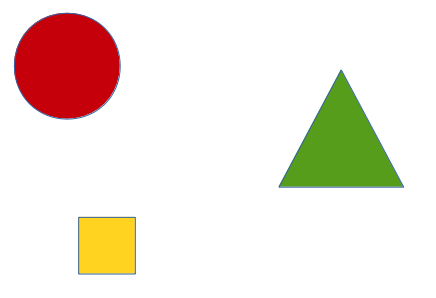
\includegraphics[width=40mm]{img/ejemplo1.png}
\caption{Señala el triángulo verde} \label{Escena de ejemplo}
\end{figure}

En nuestro caso nos centramos en una escena compuesta por figuras, pero obviamente la búsqueda de expresiones de referencia se puede emplear en diversos campos (ya veremos algún ejemplo en la memoria). Por tanto, como parte del trabajo, se desarrolló un mecanismo para la búsqueda de estas expresiones de referencia para un objeto dentro de un conjunto, sin importar la naturaleza del mismo.\\

Las expresiones de referencia se construyen a partir de la información de la que dispongamos del objeto a describir (teniendo en cuenta la que tenemos del resto de objetos) con lo cual el primer problema que abordamos es definir un mecanismo de representación del conocimiento con el cual poder manejar toda la información que podemos tener. Para ello definimos un concepto matemático que llamamos red de información. Aquí tenemos como se representa la información de la escena anterior por medio de una red de información:

\begin{figure}[H]
\centering
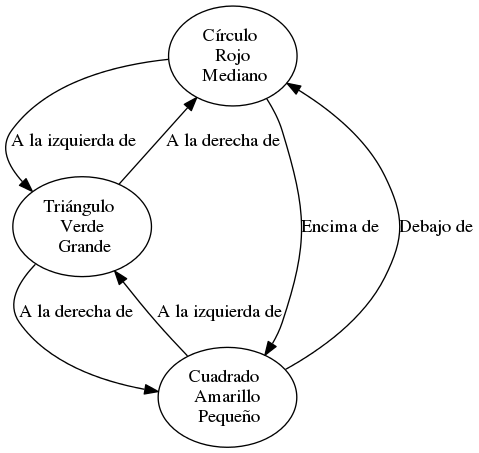
\includegraphics[scale=0.5]{img/RIejemplo1.png}
\caption{Red de información de ejemplo} \label{RI ejemplo}
\end{figure}

Al igual que sucedía en el caso de la descripción de series temporales, para un mismo objeto podemos tener varias descripciones válidas, con lo que se definió una medida de bondad para elegir la descripción que se le daba al usuario. Además, como estamos abordando un problema muy importante dentro del campo de la generación de lenguaje natural, como es el de la búsqueda de expresiones de referencia, hemos de tratar con la subjetividad inherente al lenguaje natural, con lo que empleamos la lógica difusa como mecanismo para manejar y representar esta incertidumbre.

\subsection{Mecanismo de representación de conocimientos. Redes de información.}

Una vez tenemos el dominio en el que vamos a trabajar, que si nos centramos en nuestra aplicación será una escena compuesta por figuras, tenemos que extraer la información que nos interesa de ella y modelarla para poder procesarla computacionalmente. Una estructura muy usada para estos propósitos es la estructura de grafo, al cual hay que incorpora la información de interés. Podríamos pensar que con usar un grafo etiquetado sería suficiente, puesto que simplemente queremos hablar de objetos y sus propiedades. No obstante, esta información no consistirá sólo en nombres de propiedades sino que además vendrá acompañada, en muchos problemas reales y en particular en nuestra aplicación, de unos grados de cumplimiento para estas propiedades. Así lo que hicimos fue definir una estructura matemática para modelar todo este conocimiento.\\

Como vamos a ver nuestro modelo de representación de conocimiento tendrá una estructura muy parecida a la de los grafos usuales, sólo que se agregan dos nuevos conjuntos; el conjunto de aplicaciones sobre los nodos y el de aplicaciones sobre los arcos. El grafo es un grafo dirigido, de modo que podamos almacenar la información de relaciones entre los objetos tanto simétricas como antisimétricas. El hecho de elegir los grafos nos permite aprovechar todo el potencial de los grafos y técnicas algorítmicas sobre ellos para trabajar con nuestro modelo:\\

\begin{definicion}
\label{defired}
Una \textbf{\textit{red de información}} (\textit{r.i.}) será una tripleta RI = (G,A,S) donde:\\

- G es un grafo dirigido, al que llamaremos \textbf{\textit{grafo de la red de información RI}} o simplemente \textbf{\textit{grafo}} cuando esté claro por el contexto. Siendo $V_{G}$ los vértices del grafo, $E_{G}$ sus arcos e $I_{G}$ la función de incidencia del grafo (que asocia a cada arista un par ordenado de vértices); y nos referiremos a ellos como \textbf{los objetos, conexiones y función de incidencia de la red de información RI}.\\

- A es el conjunto de propiedades que pueden tener los objetos de RI, y lo llameremos \textbf{\textit{propiedades de RI para los objetos}} o simplemente \textbf{\textit{propiedades para los objetos}} cuando esté claro por el contexto.\\
Cada $f \in A$ será una aplicación $f:V_{f} \longrightarrow B_{f}$ donde a $V_{f} \subseteq V_{G}$ (con $V_f \neq \emptyset$) lo notaremos por dom(f) (al tratarse del dominio de f como aplicación matemática) y  $B_{f}$ será el \textit{\textbf{rango de f}}  y será un conjunto cualquiera.\\

- S es el conjunto de propiedades que pueden tener las conexiones de RI, y lo llameremos \textbf{\textit{propiedades de RI para las conexiones}} o simplemente \textbf{\textit{propiedades para las conexiones}} cuando esté claro por el contexto.\\
Cada $r \in S$ será una aplicación $f:E_{r} \longrightarrow B_{r}$ donde a $E_{r} \subseteq E_{G}$ (con $E_r \neq \emptyset$ lo notaremos por dom(r) (al tratarse del dominio de r como aplicación matemática) y  $B_{r}$ será el \textit{\textbf{rango de r}}  y será un conjunto cualquiera.\\

En general a un elemento de $A \cup S$ lo llamaremos \textbf{\textit{propiedad de RI}} o simplemente \textbf{\textit{propiedad}} cuando esté claro por el contexto.
\end{definicion}

Nosotros, como ya hemos dicho, trabajamos con propiedades difusas principalmente, con lo cuál hemos de añadir un grado de verdad a cada una de las propiedades. Puede surgirnos la duda de, si hemos dejado total libertad al conjunto de valores de una propiedad, por qué no hacer simplemente que dicho conjunto sea un producto cartesiano $A\mathrm{x}I$, siendo $A$ el conjunto de valores que puede presentar una propiedad e $I$ el conjunto de grados de intensidad que puede tener un valor de dicha propiedad. Esto se debe a que hemos de exigirle algo más al $I$, y es que queríamos poder comparar grados de intensidad, entonces para ello exigimos que sobre $I$ haya definida una relación de orden. Lo que nos lleva a la siguiente definición:

\begin{definicion}
\label{defiescala}
Dado un conjunto cualquiera I y una relación de orden R sobre dicho conjunto llamaremos \textit{\textbf{escala de intensidad}} al par (I,R). Nos podemos referir a I como el conjunto base de la escela de intensidad.
\end{definicion}

Para dotar a una propiedad de intensidad lo único que hemos de hacer es tomar una escala de intensidad y que el dominio de dicha propiedad sea $A\mathrm{x}I$, donde $A$ es el conjunto de valores que puede tomar la propiedad e $I$ el conjunto base de la escala de intensidad considerada.\\

Es claro que, para el caso de las propiedades difusas usuales, este grado de intensidad será un valor en el intervalo $[0,1]$ y que por tanto esta definición de escala de intensidad parece innecesaria, pues en los números reales ya hay definidas varias relaciones de orden. Pero dar esta definición nos permite expresar la intensidad con otros elementos como pueden ser los modificadores \textit{extremadamente, muy, medio,} y  \textit{poco}.\\

\subsubsection{$\alpha$-cortes de una red de información}

En \cite{artDanielRL} podemos ver cómo pasar de un concepto difuso a una familia de conjuntos no-difusos, lo que se conoce como representación por niveles (RL), la cual tiene la ventaja de tener las mismas propiedades que las álgebras boolenas usuales. En concreto, para un conjunto difuso una RL sería el conjunto de sus $\alpha$-cortes.\\

Anteriormente hemos introducido el concepto de escala de intensidad, y esto es lo que nos permitió definir los $\alpha$-cortes de una r.i., lo que hacemos es elegir un umbral que, junto con las relaciones de orden de las distintas escalas asociadas a las propiedades de la r.i., nos da el corte.\\

Pasemos ya a ver cómo definimos un $\alpha$-corte para un r.i., lo primero que tenemos que observar es que aquellos objetos o asociaciones que no se vean afectados por dicha propiedad no se ven afectados por el corte. Por otro lado podemos establecer un corte que implique distintas propiedades.

\begin{definicion}
\label{defialfacorteprop}
Sea RI = (G, A, S) una red de información, consideramos una propiedad de la r.i. con una cierta escala de intensidad (X, R) asociada.\\

Sea $f \in A \cup S$  la propiedad considerada, y notemos por inten(v) la intensidad con la que v $\in$ dom(f), presenta su valor para la propiedad f. Entonces definimos el \textit{\textbf{$\alpha$-corte de la propiedad f de RI}} con $\alpha \in$ X como una nueva r.i. $RI_{f,\alpha} = (G_{f,\alpha}, A, R)$ donde $G_{f,\alpha}$ es un subgrafo de G definido como sigue:\\

Dado $v \in (V_{G} \cup E_{G})$, $v \in (V_{G_{f,\alpha}} \cup E_{G_{f,\alpha}})$ sii [$v \notin dom(f) \bigvee (v \in dom(f) \; \wedge \; (inten(v) \, R \, \alpha))$].
\end{definicion}

Es claro que si todos los objetos o conexiones que presenten una cierta propiedad desaparecen en el $\alpha$-corte, entonces podemos eliminar dicha propiedad de la r.i. resultante.

\begin{definicion}
\label{defisubredcondicionada}
Sea RI = (G, A, S) una red de información, consideramos un subconjunto de propiedades $P =\{f_{1},...,f_{n}\} \subseteq (A \cup S)$ cada una de ellas con una escala de intensidad ($X_{i},R_{i}$) asociada con i variando de 1 hasta n. Y sea $\alpha = (\alpha_{1},...,\alpha_{n})$ con $\alpha_{i} \in X_{i}$\\

Entonces definimos la \textit{\textbf{subred de RI condiconada a $P$ y $\alpha$}} como una nueva r.i. $RI_{P,\alpha} = (G_{P,\alpha}, A, R)$ donde $G_{P,\alpha}$ es un subgrafo de G definido como sigue:\\

Dado $v \in (V_{G} \cup E_{G})$, $v \in (V_{G_{P,\alpha}} \cup E_{G_{P,\alpha}})$ sii\\

[$(v \notin \bigcup\limits_{1}^{n}dom(f_{i})) \; \bigvee \; ((para \; cada \; f_{i} \in P \; t.q. \; v \in dom(f_{i})) \Rightarrow (inten(v) \, R_{i} \, \alpha_{i}))]$.
\end{definicion}

Como caso particular de la definición anterior, cuando podamos considerar un umbral que esté presente para todos los conjuntos base de las escalas de intensidad de todas las propiedades de la r.i., podemos dar la siguiente definición:

\begin{definicion}
Sea $RI = (G,A,S)$ una red de información, consideramos el conjunto de todas las propiedades de la r.i., $P = A \bigcup S = \lbrace p_1, ..., p_n \rbrace$ cada una de ellas con una escala de intensidad $(X_i, R_i)$, y sea $\alpha \in \overset{n}{\underset{i = 1}{\bigcap}} X_i$.\\

Entonces definimos el \textbf{$\alpha$-corte de RI} como la red de información $RI_{\alpha} = (G_\alpha, A, S)$ donde $G_\alpha$ es un subgrafo de $G$ definido como sigue:\\

Dado $v \in V_G \bigcup E_G$, $v \in V_{G_\alpha} \bigcup E_{G_\alpha}$ sii $\forall p_i \in P \; t.q. \; v \in dom(p_i), p_i(v) R_i \alpha$.
\end{definicion}

Una vez que ya tenemos modelada la información de la que disponemos en la escena el siguiente paso es buscar las expresiones de referencia para el objeto que queremos describir, esto lo veremos en la siguiente sección.

\subsection{Búsqueda de expresiones de referencia en redes de información.}

Vamos a formalizar el problema que se abordó en este trabajo para así comprender mejor el desarrollo teórico y algorítmico que sigue.\\

Partimos de una red de información compuesta por una serie de objetos $\lbrace x_1, ..., x_n\rbrace$. Entonces lo que se busca es, para cada (o uno en concreto en el caso de nuestra aplicación) objeto de esta r.i., encontrar una combinación de propiedades (o varias) $re = \lbrace p_1, ... p_n \rbrace$ de modo que el éxito referencial de esta(s) expresión(es) de referencia sea lo más grande posible.\\

Estas propiedades serán difusas con lo cual lo que hacemos es trasladar el problema a cada uno de los $\alpha$-cortes de la r.i. que tenga sentido definir (aquellos que sean distintos entre sí, que vendrán dados por el conjunto de grados distintos que presenten las propiedades de la r.i.). Estos $\alpha$-cortes se definen con un solo umbral para todas las propiedades de la r.i. original. Una vez estemos en cada nivel buscaremos expresiones de referencia $re_{ci} = \lbrace p_{ci_1}, ..., p_{ci_{m_i}} \rbrace$ que tengan éxito referencial 1 para ese objeto, en el sentido no difuso.\\

Las propiedades que se consideran en cada una de los $\alpha$-cortes de la r.i. definidos, son o bien propiedades del objeto $x_i$ a referenciar, es decir, $p_i \; t.q. \; x_i \in dom(p_i)$ (aquí hablamos sólo de pertenencia al dominio o soporte de la propiedad ya que no estamos en el caso difuso), o bien combinaciones de relaciones del corte para arcos del grafo de la r.i. con origen en $x_i$ y destino en algún $x_j$ con una rexp. de $x_j$ que no necesariamente ha de tener éxito referencial (en el sentido no difuso) para dicho objeto.\\

Finalmente, para cada una de las rexp. encontradas en los distintos niveles, lo que hacemos es medir el éxito referencia de dicha expresión de referencia con respecto a la r.i. original con información difusa, empleando la medida de éxito referencial presentada en la definición \ref{def: medida}.\\

Hemos hablado del éxito referencial de las expresiones de referencia. Pues bien, el \textbf{éxito referencial} puede definirse como la medida en la cual el conjunto de objetos (dentro de un determinado universo de discurso), a los que se les puede aplicar la expresión de referencia está compuesto únicamente por el objeto al que realmente se quiere identificar. Y teniendo en cuenta esto propusimos las siguientes propieades para una medida de éxito referencial $rs$:

\begin{enumerate}
\item $rs(re, x) = 1 \; sii \; X_{re} = \lbrace x \rbrace$.
\item Si $X_{re}(x) = 0$ entonces $rs(re, x) = 0$.
\item Si $X_{re}(y) \leq X_{re'}(y), \forall y \in X\setminus\lbrace x\rbrace$ y $X_{re}(x) \geq X_{re'}(x)$ entonces $rs(re, x) \geq rs(re', x)$.
\end{enumerate}

\subsubsection{Medidad de calidad.}

Ya hemos visto qué entendemos por éxito referencial. A continuación pasamos a introducir un modo de medir el éxito referencial cuando estamos trabajando con propiedades difusas. Esta medida, que introducimos en \cite{artReferentialSuccessCuts}, es la que empleamos en nuestra aplicación como medida de bondad de las expresiones de referencia que encontremos para un determinado objeto, escogiendo entre ellas la mejor.\\

La idea de esta medida es dar una valor en el intervalo $[0,1]$ a una expresión de referencia, $re$, con respecto a un objeto $x$ a ser referenciado. Para ello, dado que la rexp. estará formada por una colección de propiedades difusas, lo que hacemos es dividir el conjunto difuso de los objetos que se corresponden con la rexp. en sus respectivos $\alpha$-cortes y ver en cada uno de ellos si la rexp. tiene éxito referencial para el objeto en el sentido no difuso. Agregando después el valor en cada uno de los niveles.\\

En el sentido no difuso el éxito referencial de una rexp. era la medida en que ésta cumplía que $\underset{p_i \in re}{\bigcap}[[p_i]] = \lbrace x \rbrace$, siendo $x$ el objeto a referenciar y $[[p_i]] \subseteq X$ es el conjunto de objeto que tienen la propiedad $p_i$. Ahora bien, para las propiedades difusas tenemos que trabajar algo más para poder realizar este cálculo, debido a la gradualidad de las mismas.\\

Para medir la veracidad o \textit{accuracy}, cómo se adecua esa descripción a un objeto determinado, de una determinada expresión de refencia compuesta por propiedades difusas, entonces si notamos por $p_i(x)$ el grado en que la propiedad $p_i$ se da para el objeto $x$, la veracidad de la expresión de referencia $re$ para ese objeto puede calcularse como sigue:

\begin{center}
$acc_{re}(x) = \underset{i = 1}{\overset{n}{\bigotimes}} p_i(x)$
\end{center}

siendo $\bigotimes$ una t-norma. En nuestro caso la t-norma que empleamos es la del mínimo, así que lo que se muestra a continuación es para esta t-norma en concreto.\\

Antes de pasar a dar la definición nuestra medida de éxito referencial necesitaremos hacer algunas definiciones previas que mostramos a continuación:

\begin{definicion}
Dada una rexp., $re = \lbrace p_1, ..., p_n\rbrace$, compuesta por propiedades difusas y un $\alpha \in [0,1]$. Para cada propiedad $p_i \in re$, el conjunto de objetos que presentan esa propiedad con al menos grado $\alpha$, que lo notamos por $[[p_i]]_\alpha$, es el $\alpha$-corte de $X_{p_i}$.
\end{definicion}

Con esta definición podemos dar una definición de éxito referencial para una rexp. y un umbral dados.

\begin{definicion}
Sea $re = \lbrace p_1,...p_n\rbrace$ una rexp. compuesta por propiedades difusas, $\alpha \in [0,1]$ y un objeto $x \in X$. Diremos que \textbf{$re$ tiene éxito referencial en el nivel $\alpha$ para el objeto $x$} sii:

\begin{center}
$\underset{p_i \in re}{\bigcap}[[p_i]]_\alpha = \lbrace x \rbrace$
\end{center}
\end{definicion}

Esto nos lleva a la siguiente definición:

\begin{definicion}
El \textbf{conjunto de validez} de $re$ para el objeto $x$ es el conjunto de valores $\alpha$ en los que la rexp. tiene éxito referencial con respecto a $x$. Formalmente definimos este conjunto como sigue:
\begin{center}
$V_{re}^x = \left\lbrace \alpha \in [0,1] \mid \underset{p_i \in re}{\bigcap}[[p_i]]_\alpha = \lbrace x \rbrace \right\rbrace$
\end{center}
\end{definicion}

Veamos un resultado relacionado con estos conjuntos de validez:

\begin{proposicion}
Si $V_{re}^x \neq \emptyset$ entonces es un intervalo.
\end{proposicion}

Lo que nos está diciendo esta proposición es que una rexp., $re$, para la cual $V_{re}^x \neq \emptyset$ comienza a tener éxito referencial en un determinado valor $\alpha_1 \in [0,1]$ y deja de tenerlo en otro (menor o igual) $\alpha_2 \in [0,1]$, con:

\begin{center}
$\alpha_1 = sup(V_{re}^x)$\\
$\alpha_2 = inf(V_{re}^x)$
\end{center}

\begin{proposicion}
\label{prop3.7}
Sea $re$ una expresión de referencia con propiedades difusas y $X_{re}$ el conjunto difuso de objetos que satisfacen $re$. Sea $X = \lbrace x_1, x_2, ..., x_m \rbrace$ con $m \geq 2$ de modo que $X_{re}(x_i) \geq X_{re}(x_{i+1}) \forall 1 \leq 1 < m$. Sea $x \in X$ tal que $V_{re}^x \neq \emptyset$. Entonces:
\begin{enumerate}
\item $x = x_1$.
\item $\alpha_1 = X_{re}(x) > X_{re}(x_2) = \alpha_2$.
\end{enumerate}
\end{proposicion}

Por lo tanto, cuanto más grande sea $\alpha_1$, mayor será la veracidad de la rexp. para $x$. Y cuanto menor sea $\alpha_2$, menor será esta veracidad para el resto de objetos. En base a esto damos la siguiente definición de medida de éxito referencial, para una rexp. $re$ y un objeto $x$:

\begin{definicion}
\label{def: medida}
$rs(re, x) = \left\lbrace 
\begin{array}{ll}
      \alpha_1(\alpha_1 - \alpha_2) \; \mathrm{si} \; V_{re}^x \neq \emptyset\\      
      0 \; \mathrm{en \, otro \, caso}\\
\end{array} \right.$
\end{definicion}

Y así tenemos una nueva propuesta de medida de éxito referencial para dominios con información difusa. Así por ejemplo, en la siguiente escena tenemos un círculo verde puro y un círculo amarillo-verdoso (0.7 amarillo + 0.3 verde). Entonces, aunque las expresiones de referencia ``el círculo'' y ``el objeto azul'' son válidas para describir al círculo, la primera será mejor pues siempre es válida y la segunda es válida a partir de grado 0.3.

\begin{figure}[H]
\centering
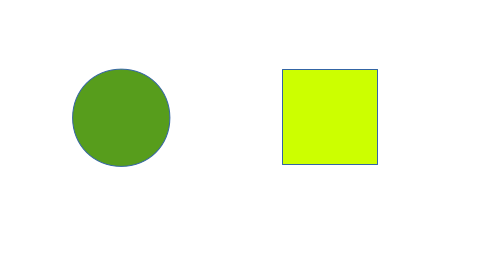
\includegraphics[scale=0.3]{img/ejemploMedidaBondad.png}
\caption{Ejemplo medida de éxito referencial}
\end{figure}

\subsubsection{Diseño del algoritmo}

Una vez que tenemos la información modelada por medio de una red de información, que nos permite que sea tratable por un ordenador, y conocemos la medida de calidad que buscamos maximizar en las expresiones de referencia que encontremos, tenemos que realizar la búsqueda de dichas expresiones dentro de la r.i.. Para ello diseñamos un algoritmo que realiza un refinamiento iterativo de las soluciones, que va aumentando la profundidad de su búsqueda según lo necesita.\\

El algoritmo intenta obtener las expresiones de referencia lo más cortas posibles; de modo que va probando con expresiones de referencia cada vez más largas (o de mayor coste en nuestro caso) hasta encontrar una que tenga éxito referencial (probaremos hasta un tope máximo de tamaño).\\

Las nuevas propiedades que le añadimos a cada nodo serán combinaciones de relaciones que tenga el nodo con sus vecinos en la red de información, con expresiones de referencia que sean apropiadas para el vecino o vecinos asociados por esas relaciones. Cabe señalar que estas descripciones de los vecinos deberán tener veracidad para ese vecino, es decir, deben poder aplicarse al vecino, pero no tienen que tener éxito referencial; es decir, pueden ser aplicables a otros nodos de la red de información. Además, en el caso de las propiedades de coste 1, éstas son las propiedades internas del nodo, como por ejemplo el color y el tamaño de los elementos de nuestra escena.\\

Lo que hacemos, como es usual cuando se está trabajando con información difusa, es obtener una serie de redes de información con información no difusa a partir de la r.i. que describe la escena. Estos niveles son $\alpha$-cortes de la r.i.. De este modo el primer paso fue diseñar un algoritmo que genere expresiones de referencia para objetos con propiedades no difusas y luego se empleó este algoritmo en cada uno de los niveles en los que hemos descompuesto nuestro problema difuso; siguiendo una estrategia divide y vencerás. Así nuestro algoritmo no difuso puede ser descrito por el siguiente diagrama de flujo:

\begin{figure}[H]
\centering
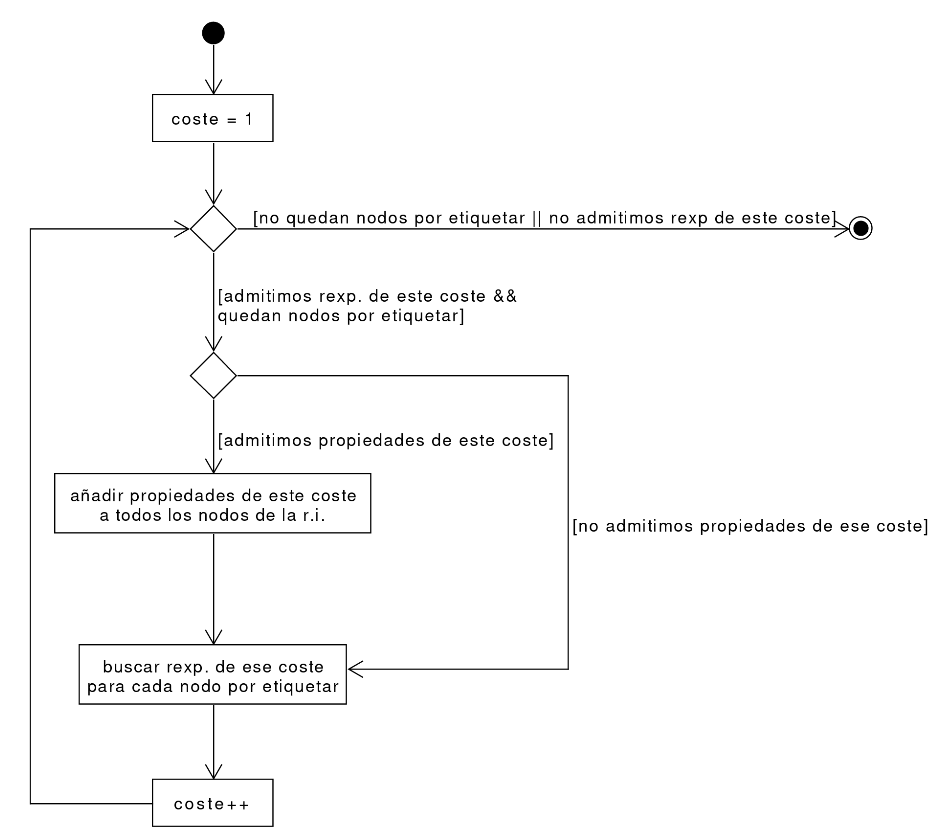
\includegraphics[scale=0.5]{img/diagramaFlujoAlgCrisp.png}
\caption{Diagrama de flujo para el algoritmo base}
\end{figure}

Para comprobar si un nodo tiene una expresión de referencia de un coste dado, lo que hacemos es elaborar todas las combinaciones posibles de propiedades del nodo que alcancen como coste total ese coste y ver si, en el sentido no difuso, esta combinación constituye una expresión de referencia con éxito referencial para ese nodo, es decir, que no haya otro nodo de la r.i. que tenga las propiedades que conforman esa expresión de referencia.\\

Señalar que estamos hablando en singular, pero como ya hemos dicho anteriormente para un nodo podemos encontrar diversas expresiones de referencia con el mismo coste. Además, en el caso en que sólo quisiéramos encontrar una expresión de referencia para cada nodo, en lugar de encontrar todas las posibles dentro del peso mínimo necesario, en cuanto un nodo está etiquetado su peso puede propagarse a aquellos vecinos que tengan una referencia única hacia él. Es decir, si un nodo queda con peso 1 con la expresión de referencia ``círculo'', el único vecino suyo que esté a la izquierda tiene automáticamente la expresión de referencia ``el que está a la izquierda de un círculo'' o, si es un triángulo y obligamos a incluir el tipo del objeto en la rexp. ``triángulo a la izquierda de un círculo''.\\

Este algoritmo lo aplicamos sobre cada uno de los $\alpha$-cortes de la red de información con propiedades difusas con la que estemos trabajando, los $\alpha$-cortes que consideramos son aquellos dados por los grados distintos que presenten las propiedades y relaciones de la r.i.. No tiene sentido considerar otros ya que entre uno de los grados que estén presentes en lar r.i. y el siguiente no cambiará el $\alpha$-corte resultante.

El diagrama de flujo para el algoritmo con el que buscamos y seleccionamos expresiones de referencia para los nodos de una r.i. con información difusa sería el siguiente:

\begin{figure}[H]
\centering
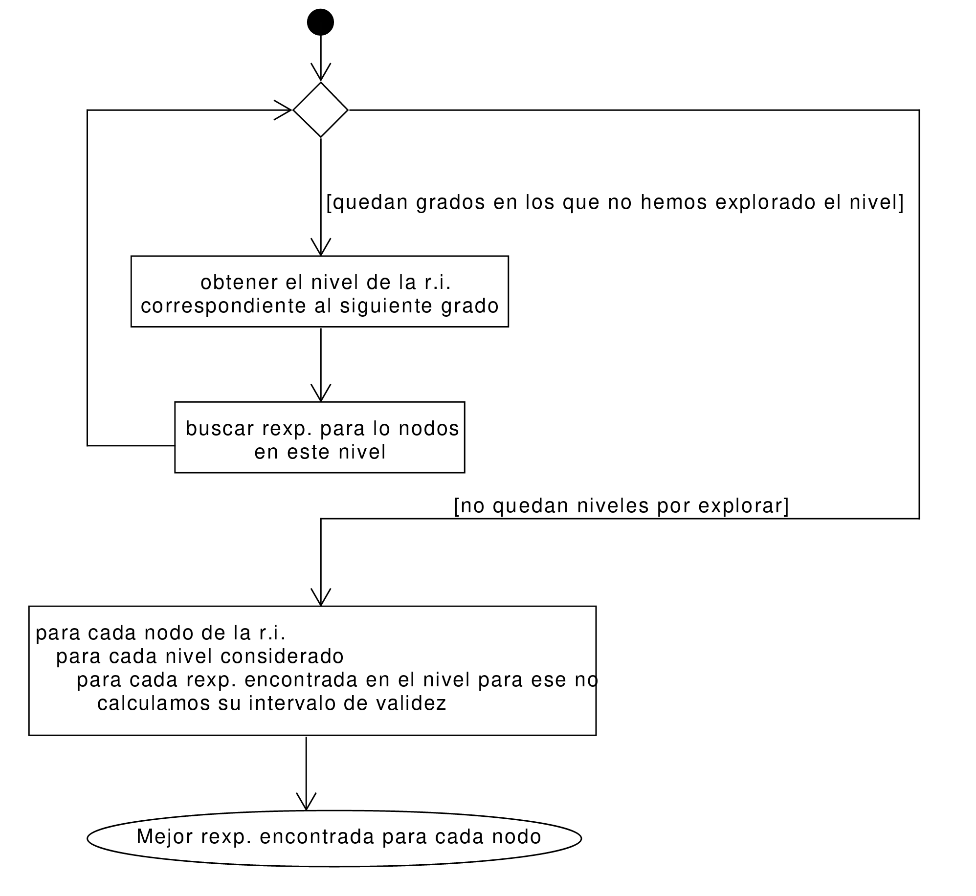
\includegraphics[scale=0.5]{img/diagramaFlujoAlgFuzzy.png}
\caption{Diagrama de flujo para el algoritmo para información difusa}
\end{figure}

Veamos un ejemplo para la siguiente escena cuya información puede modelarse por medio de una r.i. como sigue:

\begin{figure}[H]
\subfloat[escena]{
\includegraphics[width=0.55\textwidth]{img/ejemploAlgoritmoNoDifuso.png}}
\subfloat[r.i.]{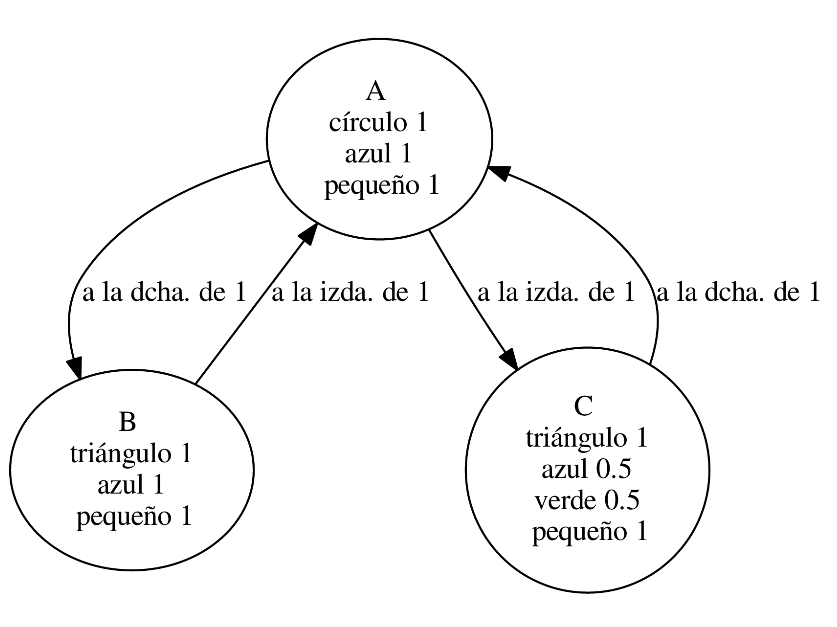
\includegraphics[width=0.6\textwidth]{img/riEjemploAlgoritmoNoDifuso.png}}
\end{figure}

Entonces en este caso tan trivial se establecerían dos $\alpha$-cortes distintos, el de grado 0.5 y el de grado 1, que se corresponderían con las dos r.i. siguientes:\\

\begin{figure}[H]
\subfloat[0.5-corte]{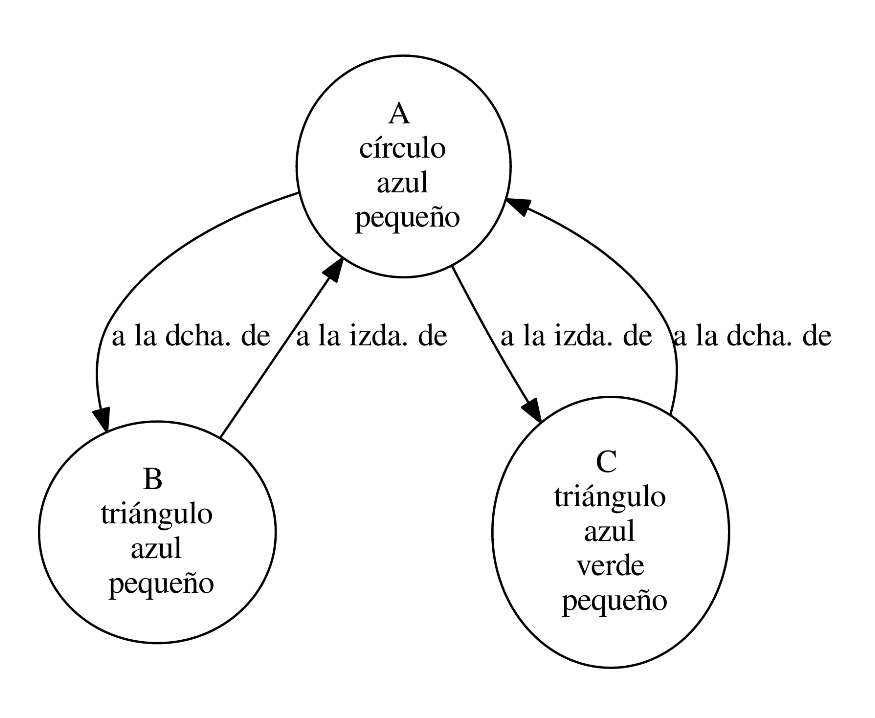
\includegraphics[width=0.5\textwidth]{img/riEjemploAlgoritmoDifusoCorte05.png}}
\subfloat[1-corte]{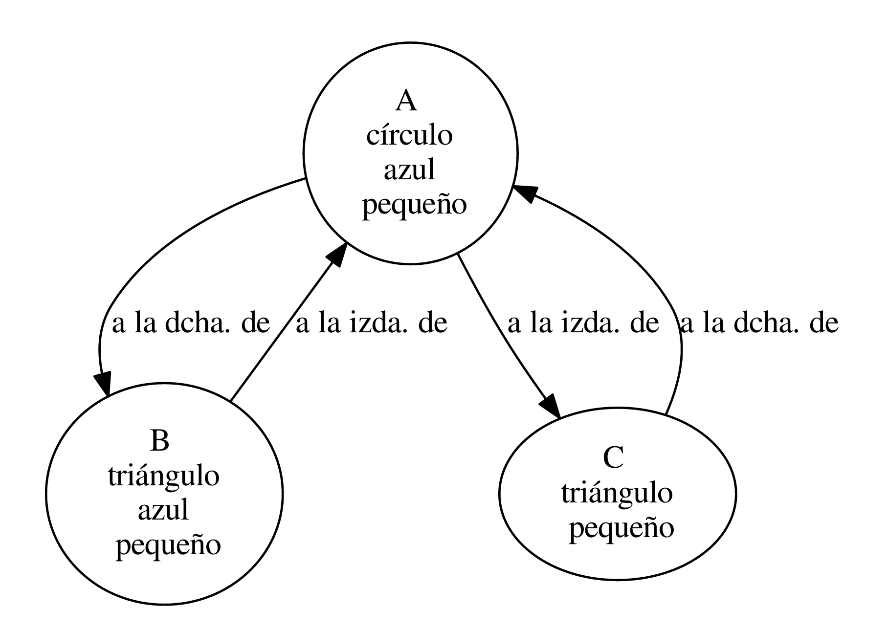
\includegraphics[width=0.5\textwidth]{img/riEjemploAlgoritmoDifusoCorte1.png}}
\end{figure}

Entonces estas serían las expresiones de referencia que se encontrarían para cada nodo en cada uno de los niveles, aplicando el algoritmo no difuso en ambos. También mostramos el intervalo de grados donde tendrían validez dichas expresiones junto con la medida de bondad asociada:

\begin{table}[H]
\centering
\caption{Expresiones de referencia encontradas}
\label{my-label}
\begin{tabular}{|l|l|l|l|l|}
\hline
Corte                                          & Nodo & Rexp. encontradas                      & Intervalo   & Medida \\ \hline
\multirow{3}{*}{0.5-corte}                     & A    & {[}círculo{]}                          & {[}0,1{]}   & 1      \\ \cline{2-5} 
                                               & B    & {[}triángulo, a la izda. de círculo{]} & {[}0,1{]}   & 1      \\ \cline{2-5} 
                                               & C    & {[}triángulo, verde{]}                 & {[}0,0.5{]} & 0.25   \\ \hline
\multicolumn{5}{|l|}{}                                                                                                \\ \hline
\multicolumn{1}{|c|}{\multirow{3}{*}{1-corte}} & A    & {[}círculo{]}                          & {[}0,1{]}   & 1      \\ \cline{2-5} 
\multicolumn{1}{|c|}{}                         & B    & {[}triángulo, azul{]}                  & {[}0.5,1{]} & 0.5    \\ \cline{2-5} 
\multicolumn{1}{|c|}{}                         & C    & {[}triángulo, a la dcha. de círculo{]} & {[}0,1{]}   & 1      \\ \hline
\end{tabular}
\end{table}

Aquí podemos observar también cómo funciona nuestra medida, nos dice que las expresiones de referencia para los triángulos que usan el color son peores que aquellas que, siendo algo más largas, emplean las posiciones relativas entre los triángulos y el círculo, ya que estas son más concretas que hablar del color que, en uno de los dos triángulos no está del todo claro.\\

\subsection{Aplicación Android: Touch and Learn}

Ya hemos dicho de qué trata nuestra aplicación y como sabemos nosotros trabajamos con información difusa. En concreto los componentes de la escena que se le presenta al niño que presentan información difusa son: el color, el tamaño y las posiciones relativas entre las figuras. La forma o el tipo de figura no será difuso, podríamos decir que sí lo es, pero el tipo que le asignamos a una figura será único con grado 1. Pues bien vamos a ver cómo representamos está información con incertidumbre en nuestra aplicación.

Los tamaños con los que trabajamos en nuestra aplicación están en unidad de píxels de pantalla y etiquetaremos cada figura según su radio en esta medida, variando entre 50 y 150 píxels. Cuando hablamos de radio para un triángulo o un cuadrado, hablamos del radio del círculo en el que el triángulo está circunscrito o del radio del círculo que está inscrito en el cuadrado.\\

Las etiquetas que le asociamos a una figura según su radio vienen dadas por la siguiente partición difusa del rango de tamaños en los que se moverán las figuras:

\begin{figure}[H]
\centering
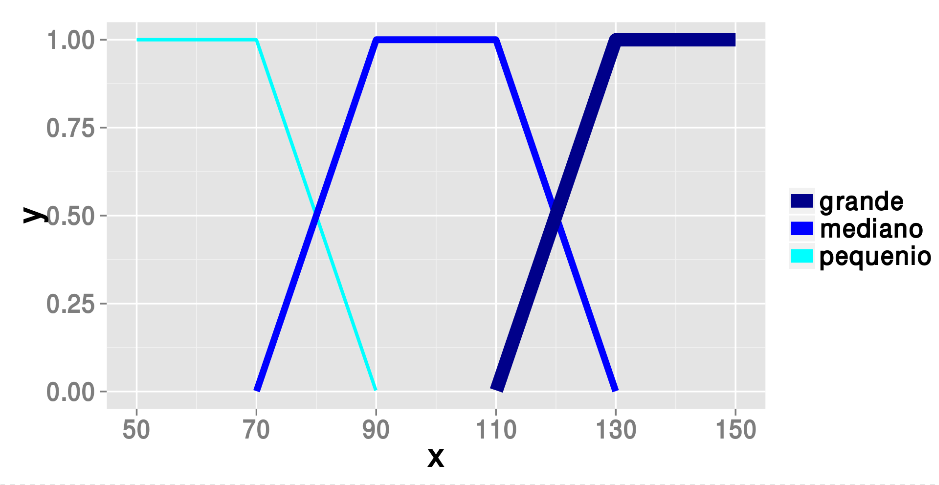
\includegraphics[width = \textwidth]{img/partitionTam.png}
\caption{Partición difusa para el tamaño de las figuras}
\end{figure}

Ahora para calcular la posición relativa de una figura con respecto a la otra medimos el ángulo que forma el centro de la otra figura con respecto al centro de la figura a la que queremos calcular sus posiciones relativas. Entonces la partición difusa que haremos para establecer las relaciones espaciales de una figura con otra vendrán dadas por la siguiente partición en el intervalo [0,360]:\\

\begin{figure}[H]
\centering
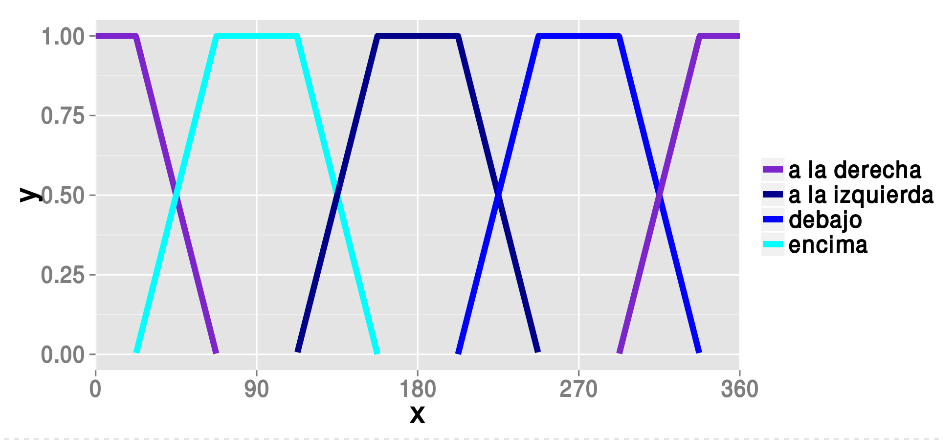
\includegraphics[width = \textwidth]{img/partitionRelPos.png}
\caption{Partición difusa para la posición relativa entre figuras}
\end{figure}

Ahora pasemos al color, para etiquetar el color de las figuras nos inspiramos en las particiones difusas que se hacen sobre el cono del espacio HSV de color en \cite{artDaniHSV}. Nosotros no jugamos con todo el espectro de etiquetas que en este artículo se plantea si no que distinguimos entre colores con saturación y brillo con valor 1, es decir los colores más brillantes y saturados, y la escala de grises que obtenemos si bajamos la saturación a cero, fijamos un número cualquiera para el hue (H) del color (en nuestro caso fijamos el cero) y movemos el brillo del color en el [0,1]. Así los colores con saturación máxima se etiquetaran por un lado y lo colores con saturación nula por otro, según las siguientes particiones difusas:\\

\begin{figure}[H]
\centering
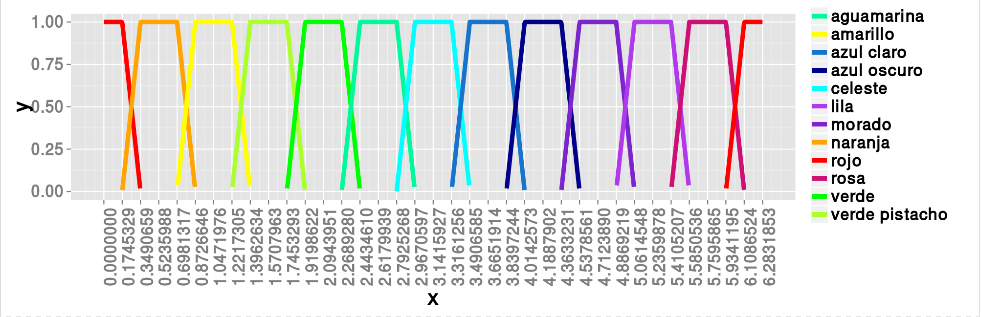
\includegraphics[width = \textwidth]{img/partitionColor.png}
\caption{Partición difusa para los colores de las figuras}
\end{figure}

\begin{figure}[H]
\centering
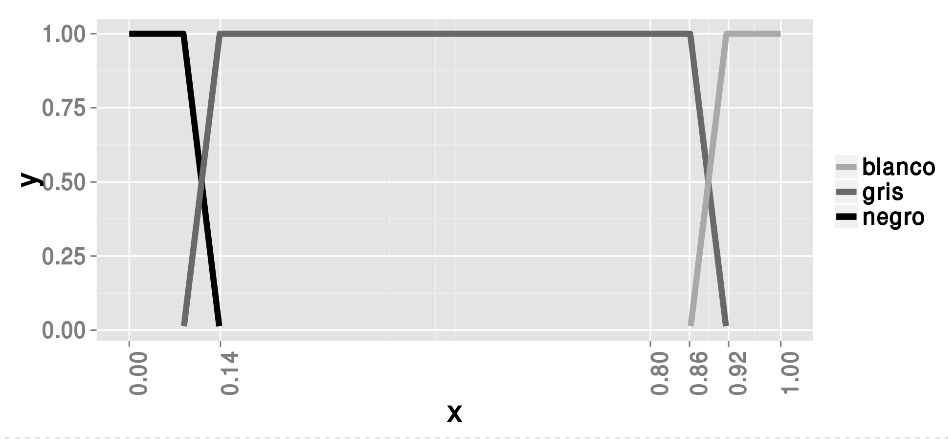
\includegraphics[width = \textwidth]{img/partitionGrey.png}
\caption{Partición difusa para la escala de grises de los colores de las figuras}
\end{figure}

Hemos de señalar que aquí aparecen colores que quizás sean difíciles de identificar por un niño como el color aguamarina, pero esto es sólo la gama de colores que empleamos en nuestra aplicación a modo de muestra. Podríamos haber definido otra partición difusa distinta con otras etiquetas distintas, el funcionamiento de la aplicación, y del algoritmo en particular, no se verían afectados.\\

Para ver una demostración del funcionamiento de la aplicación podemos visitar \href{https://www.youtube.com/watch?v=sfQNCcHsYu8}{el vídeo} que se realizó para tal efecto durante el desarrollo del Trabajo Fin de Grado.
\newpage

\nocite{*}
\bibliographystyle{unsrt}
\bibliography{biblio}
\end{document}